% --------------------------------------------------------------
% This is all preamble stuff that you don't have to worry about.
% Head down to where it says "Start here"
% --------------------------------------------------------------
 
\documentclass[12pt]{article}
 
\usepackage[margin=1in]{geometry} 
\usepackage{amsmath,amsthm,amssymb}
 
\newcommand{\N}{\mathbb{N}}
\newcommand{\Z}{\mathbb{Z}}
\newenvironment{abs}[2][Part I Abstract]{\begin{trivlist}
\item[\hskip \labelsep {\bfseries #1}\hskip \labelsep {\bfseries #2}]}{\end{trivlist}}

\newenvironment{p1}[2][Part II Motivation]{\begin{trivlist}
\item[\hskip \labelsep {\bfseries #1}\hskip \labelsep {\bfseries #2}]}{\end{trivlist}}

\newenvironment{p2}[2][Part III Data and Software Tools]{\begin{trivlist}
\item[\hskip \labelsep {\bfseries #1}\hskip \labelsep {\bfseries #2}]}{\end{trivlist}}

\newenvironment{p3}[2][Part IV Methods]{\begin{trivlist}
\item[\hskip \labelsep {\bfseries #1}\hskip \labelsep {\bfseries #2}]}{\end{trivlist}}

\newenvironment{p4}[2][Part V Results and Evaluation]{\begin{trivlist}
\item[\hskip \labelsep {\bfseries #1}\hskip \labelsep {\bfseries #2}]}{\end{trivlist}}

\newenvironment{p5}[2][Part VI Discussion and Future Work]{\begin{trivlist}
\item[\hskip \labelsep {\bfseries #1}\hskip \labelsep {\bfseries #2}]}{\end{trivlist}}

\newenvironment{p6}[2][References]{\begin{trivlist}
\item[\hskip \labelsep {\bfseries #1}\hskip \labelsep {\bfseries #2}]}{\end{trivlist}}

\usepackage{graphicx}
\graphicspath{{./}}

\begin{document}
 
% --------------------------------------------------------------
%                         Start here
% --------------------------------------------------------------
 
\title{San Francisco Crime Study}
\author{Yunzhong He (204010749) Zhinan Guan (004118232)}
\maketitle

\begin{abs}{}
\item{}
For this project we performed data minings and visualizations on San Francisco's crime data from 2003 to 2015, in order to find patterns in the space-time distributions of different types of crimes. And we want to predict the probability distribution of each crime occurance. We first performed feature selection on street names using decision trees, and obtained the most meaningful names in terms of separating different kinds of crimes. Then we used logistic regression, with respect to time, GPS coordinate and the features selected in the previous step, to learn the likelihood function of different crimes. We compared our results with Nearest Neighbor classifier using time and location, and showed that our approach significantly reduced the log loss. Eventually, using our learned results we were able to generate heat maps for different crimes throughout San Francisco.
\end{abs}

\begin{p1}{}
\item{}
San Francisco was know for its numerous crimes in the past. Nowadays, the growing housing shortage,  inequality of wealth lead to many crimes in the city. Given time and location of all the crimes in nearly 12 years in San Francisco, we want to use machine learning to study the data, and to find the key factors in terms of time and location that causes different crimes. We got the idea of our project from an ongoing competition on Kaggle.com. 
\end{p1}

\begin{p2}{}
\item{}
We obtained all the data of this project from Kaggle[1], including a train dataset and a test dataset in cvs format. Original features of each crime in the datasets are: Timestamp, Day of Week, District, Address, Latitude, Longitude. To make the address useful, we extracted only the street name from the address rather than using the exact address. We used all these features to learn the data.\\\\
The project is implemented in Python, with several third party packages. We used "numpy" package while preprocessing the data, "scikit-learn" package for the data mining algorithms, and gmplot to visualize the results on San Francisco map. 
\end{p2}

\begin{p3}{}
\item{\textbf{IV.1 Feature Selection with Random Forrest\\}}
From the dataset we are given the district and street names of all the crime occurrences. Using bag-of-word model[2] we can encode them into binary vectors as part of our feature. But with the size of our dataset, the computation is going to take very long time given the dimension of our feature space. More importantly, the resultant vector of bag-of-words encoding is very sparse -- for a vector of 500+ entries representing bag-of-words encoding of one data point, at most two entries will be 1, because there is only one district and one street name for each crime incident.\\\\
To address this issue, we want to filter out streets that are not very informative in terms of crime classification. Limiting our bag-of-words model to contain only 10 words for street names, we want to find a subset S, of the set of all streets W, that maximizes the information gain. We have
\begin{align*}
	S^* = argmax_{S \subset W} \sum_i^N log(p(x_i|S)) p(S)
\end{align*}
This is thus very similar to decision tree learning, except that we want to pick the top 10 features, rather than picking one at each depth. We used an ensemble model, the Extremely Randomized Trees[3] to solve the problem. It basically uses many randomized decision trees, and compute the feature importance based on its frequency of being picked.\\

\item{\textbf{IV.2 Classification Using Logistic Regression\\}}
Since the resulting dimension of our feature space after feature selection is 101, it is reasonable to believe that the data can be well-separated with linear decision boundaries. So we chose logistic regression as our classification due to its simplicity. We also ran cross validation with different regularization parameters and picked the best parameter.
\end{p3}

\begin{p4}{}
\item{\textbf{V.1 Feature Selection Results}\\}
Running the feature selection process for districts and streets, below are the top 10 names we found.
\begin{center}
	\begin{tabular}{||c||} 
		\hline
	   	Name \\
		\hline
		BLAKE\\
		\hline
		ELM \\
		\hline
		FAIR\\
		\hline
		TUBBS\\
		\hline
		TARA\\
		\hline
		PARKRIDGE\\
		\hline
		SANTAPAULA\\
		\hline
		ELLINGTON\\
		\hline
		PEARL\\
		\hline
		FLOWER\\
		\hline
	\end{tabular}
	{\\fig.1 best names}
\end{center}
From the table we can see that in general districts are more informative than streets. And since we are using decision trees, this should not be a result of districts having higher frequencies to appear in our dataset than streets. We further normalized our data and ran the same algorithm, and obtained the same results. But notice that Mission Ave is more informative than some districts, which is an interesting observation.\\

\item{\textbf{V.2 Log Loss on Testing Data}\\}
We followed Kaggle's criteria and used log-likelihood given by the equation below to evaluate our predication accuracy.
\begin{align*}
	logloss = -\sum_i^N \sum_j^M y_{ij} log (p_{ij})
\end{align*}
For the testing dataset Kaggle provided, we ran our trained classifier and predicted the probability of each entry. The outcomes are formatted and submitted to Kaggle, and we obtained \textbf{2.81} log loss, which beats around 70\% of the participants. We also ran a nearest neighbor classifier with respect to the raw time and location data given to compare the results. Below is a table of different results.
\begin{center}
	\begin{tabular}{||c c||} 
		\hline
	   	Algorithm & Log Loss \\
		\hline
		Logistic regression with feature selection & 2.56 \\
		\hline
		Kaggle median & 2.60\\
		\hline
		Logistic regression without selected features& 2.86 \\
		\hline
		Nearest Neighbor & 28.89 \\
		\hline
		Prediction based on prior only & 32.8 \\
		\hline
	\end{tabular}
	{\\fig.2 results comparison}
\end{center}
\item{\textbf{V.3 Data Visualization}\\}
\\ 
The heat-maps below show an visualization of  our prediction distribution on test dataset comparing with the actual distribution on training dataset for two sample crime categories. Based on the visualization, we can see that our prediction is really similar to the actual distribution from the training dataset in both examples based on the relative red vs yellow vs green areas. \\
\\
\newpage
\begin{center}
Heat-map of Actual Training Dataset for \textbf{Larceny/Theft}:\\
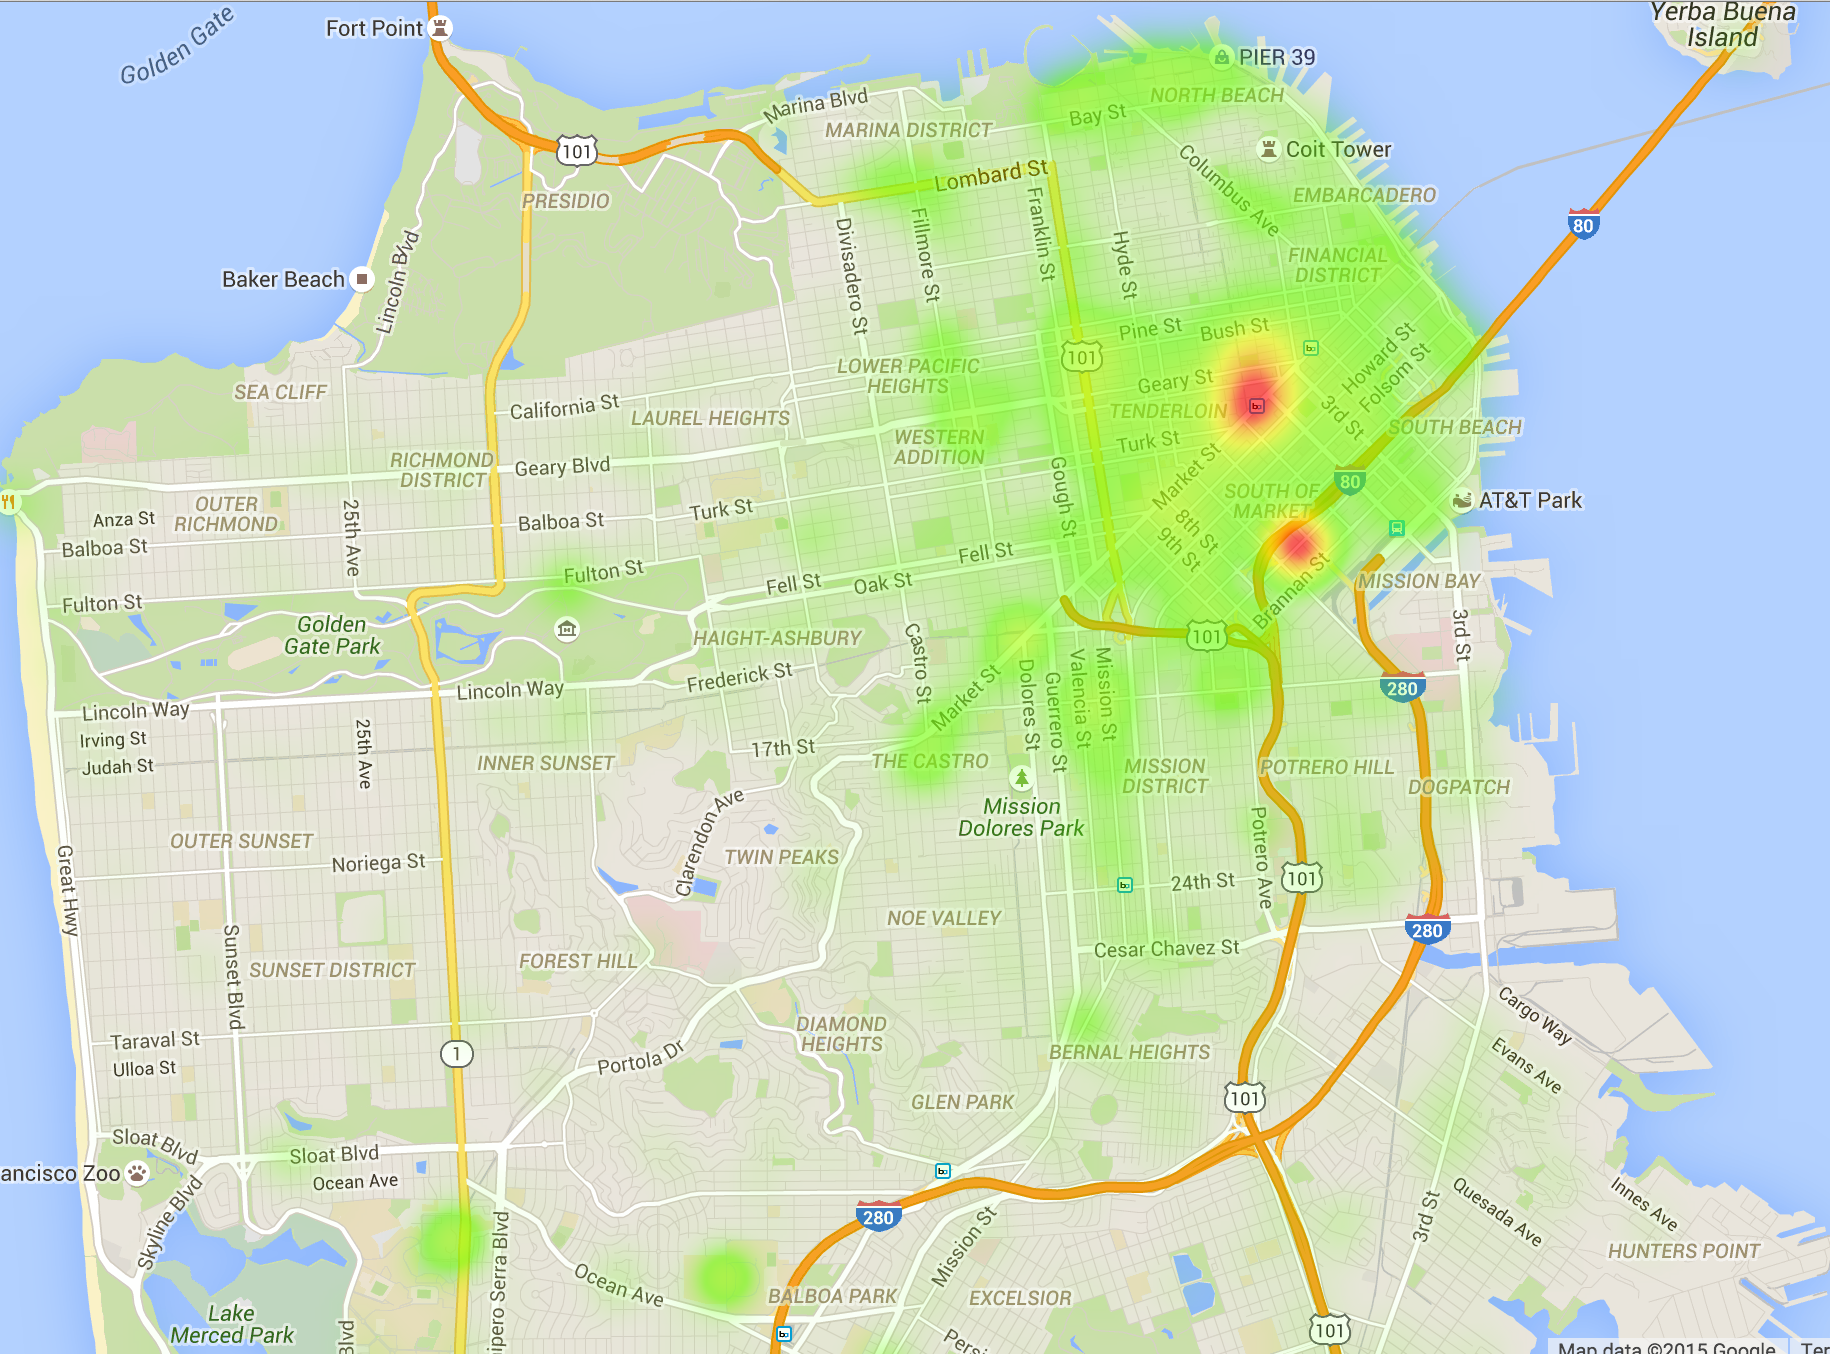
\includegraphics[height=10cm]{LARCENY_THEFT_train.png}
\\
Heat-map of Test Prediction for \textbf{Larceny/Theft}:\\
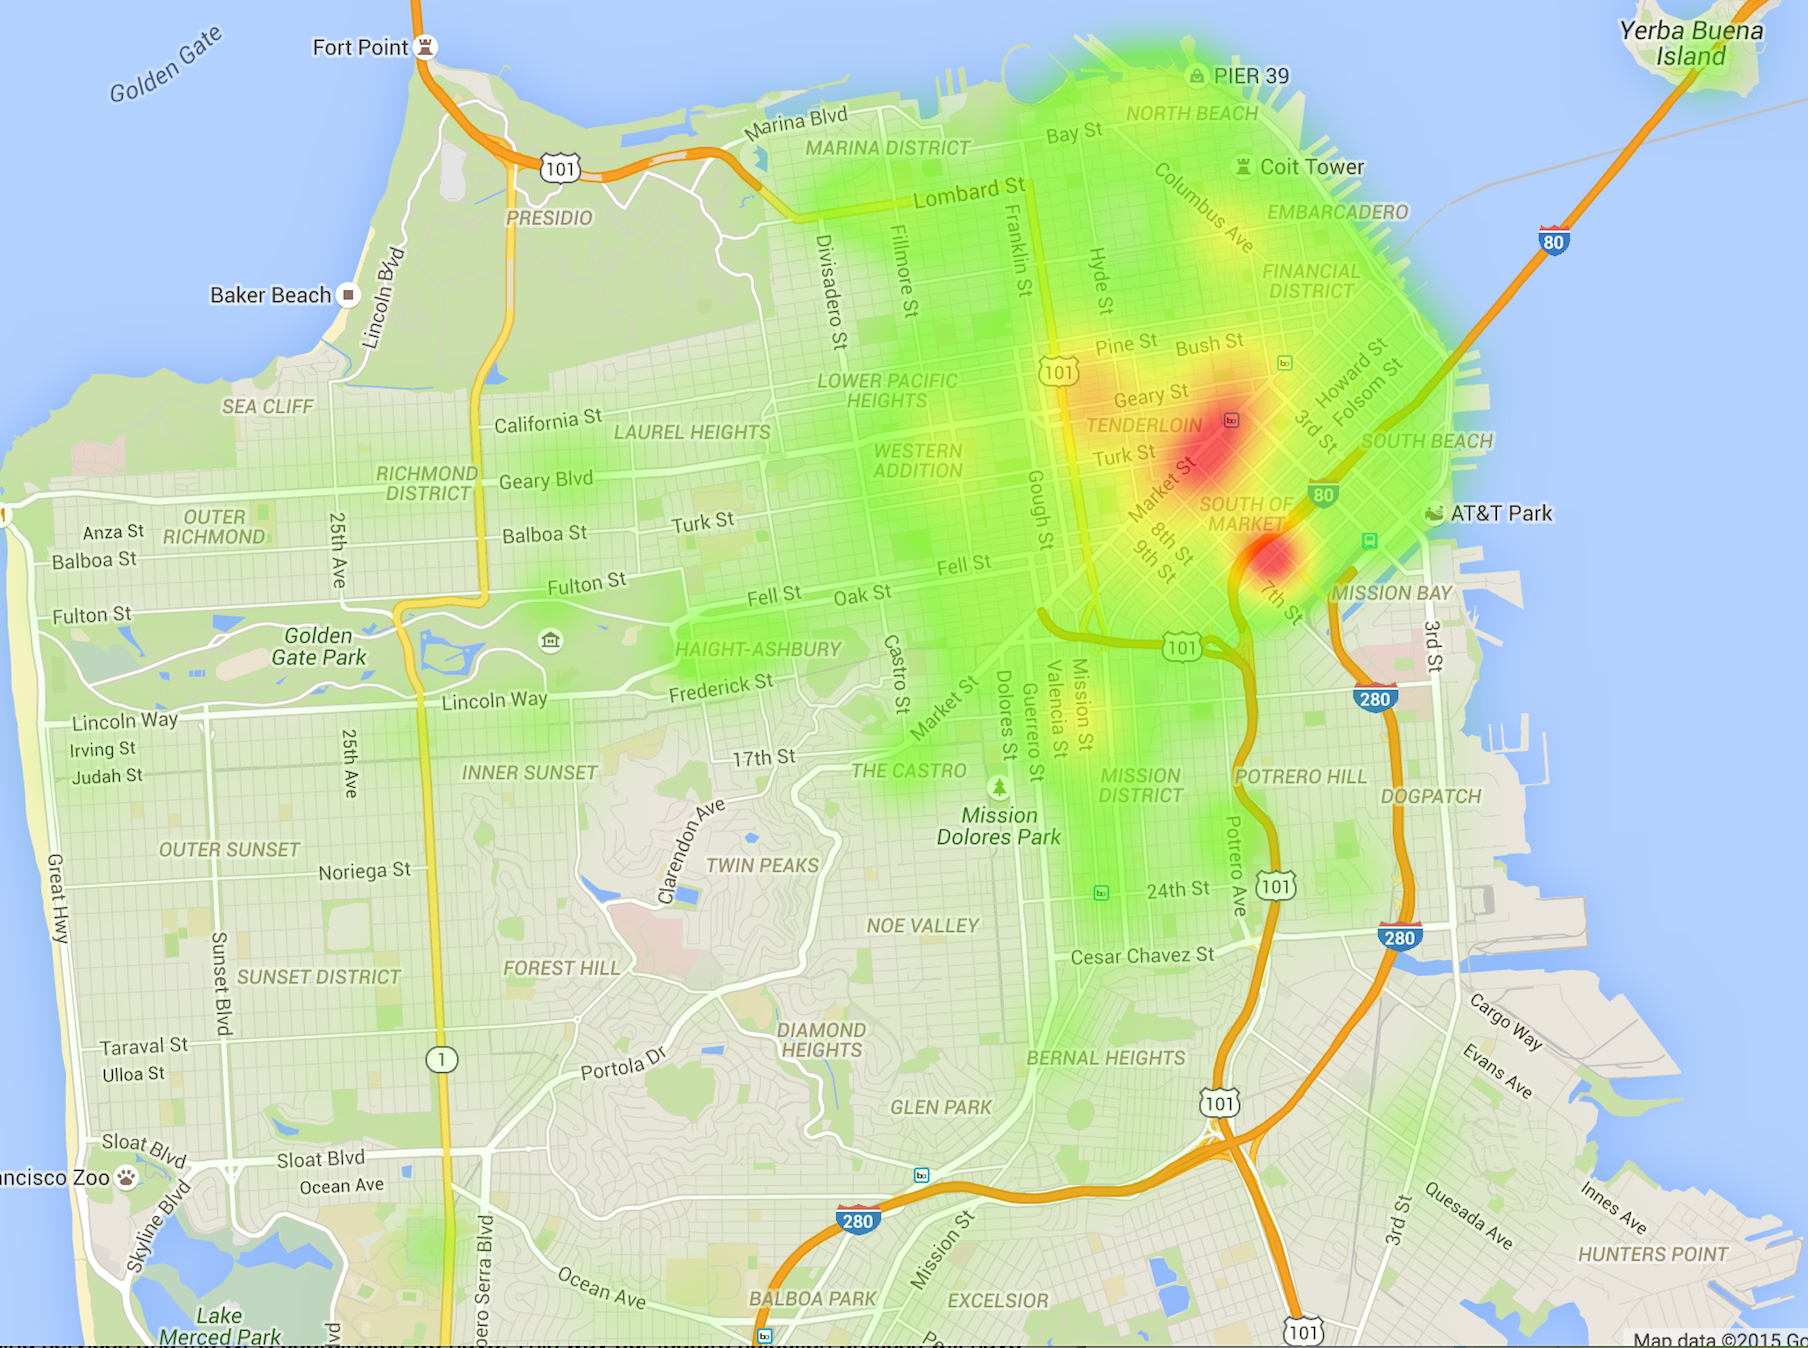
\includegraphics[height=10cm]{LARCENY_THEFT_test.png}
\end{center}
\newpage
\begin{center}
Heat-map of Actual Training Dataset for \textbf{Assault}:\\
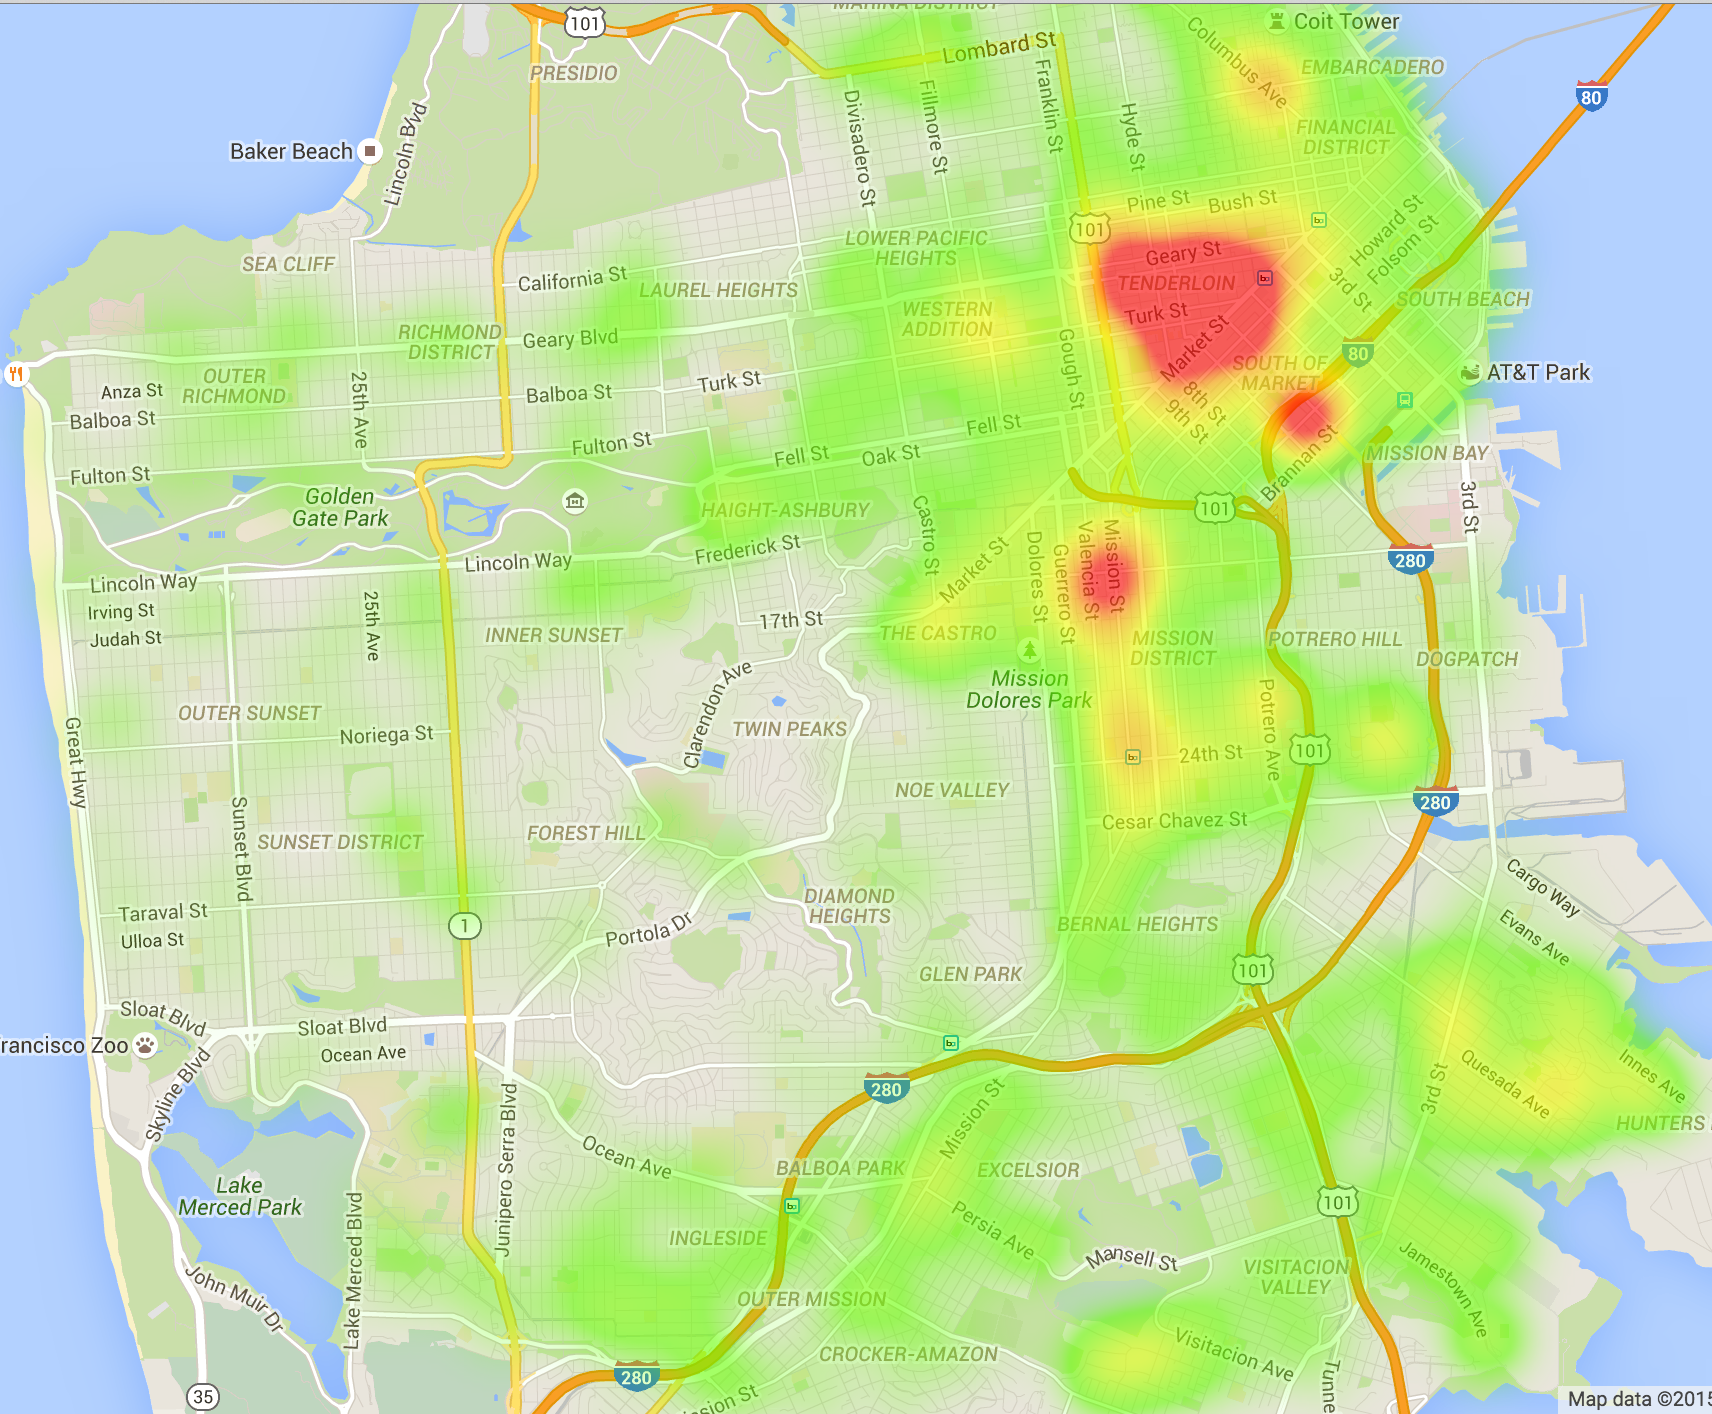
\includegraphics[height=10cm]{ASSAULT_train.png}
\\
Heat-map of Test Prediction for \textbf{Assault}:\\
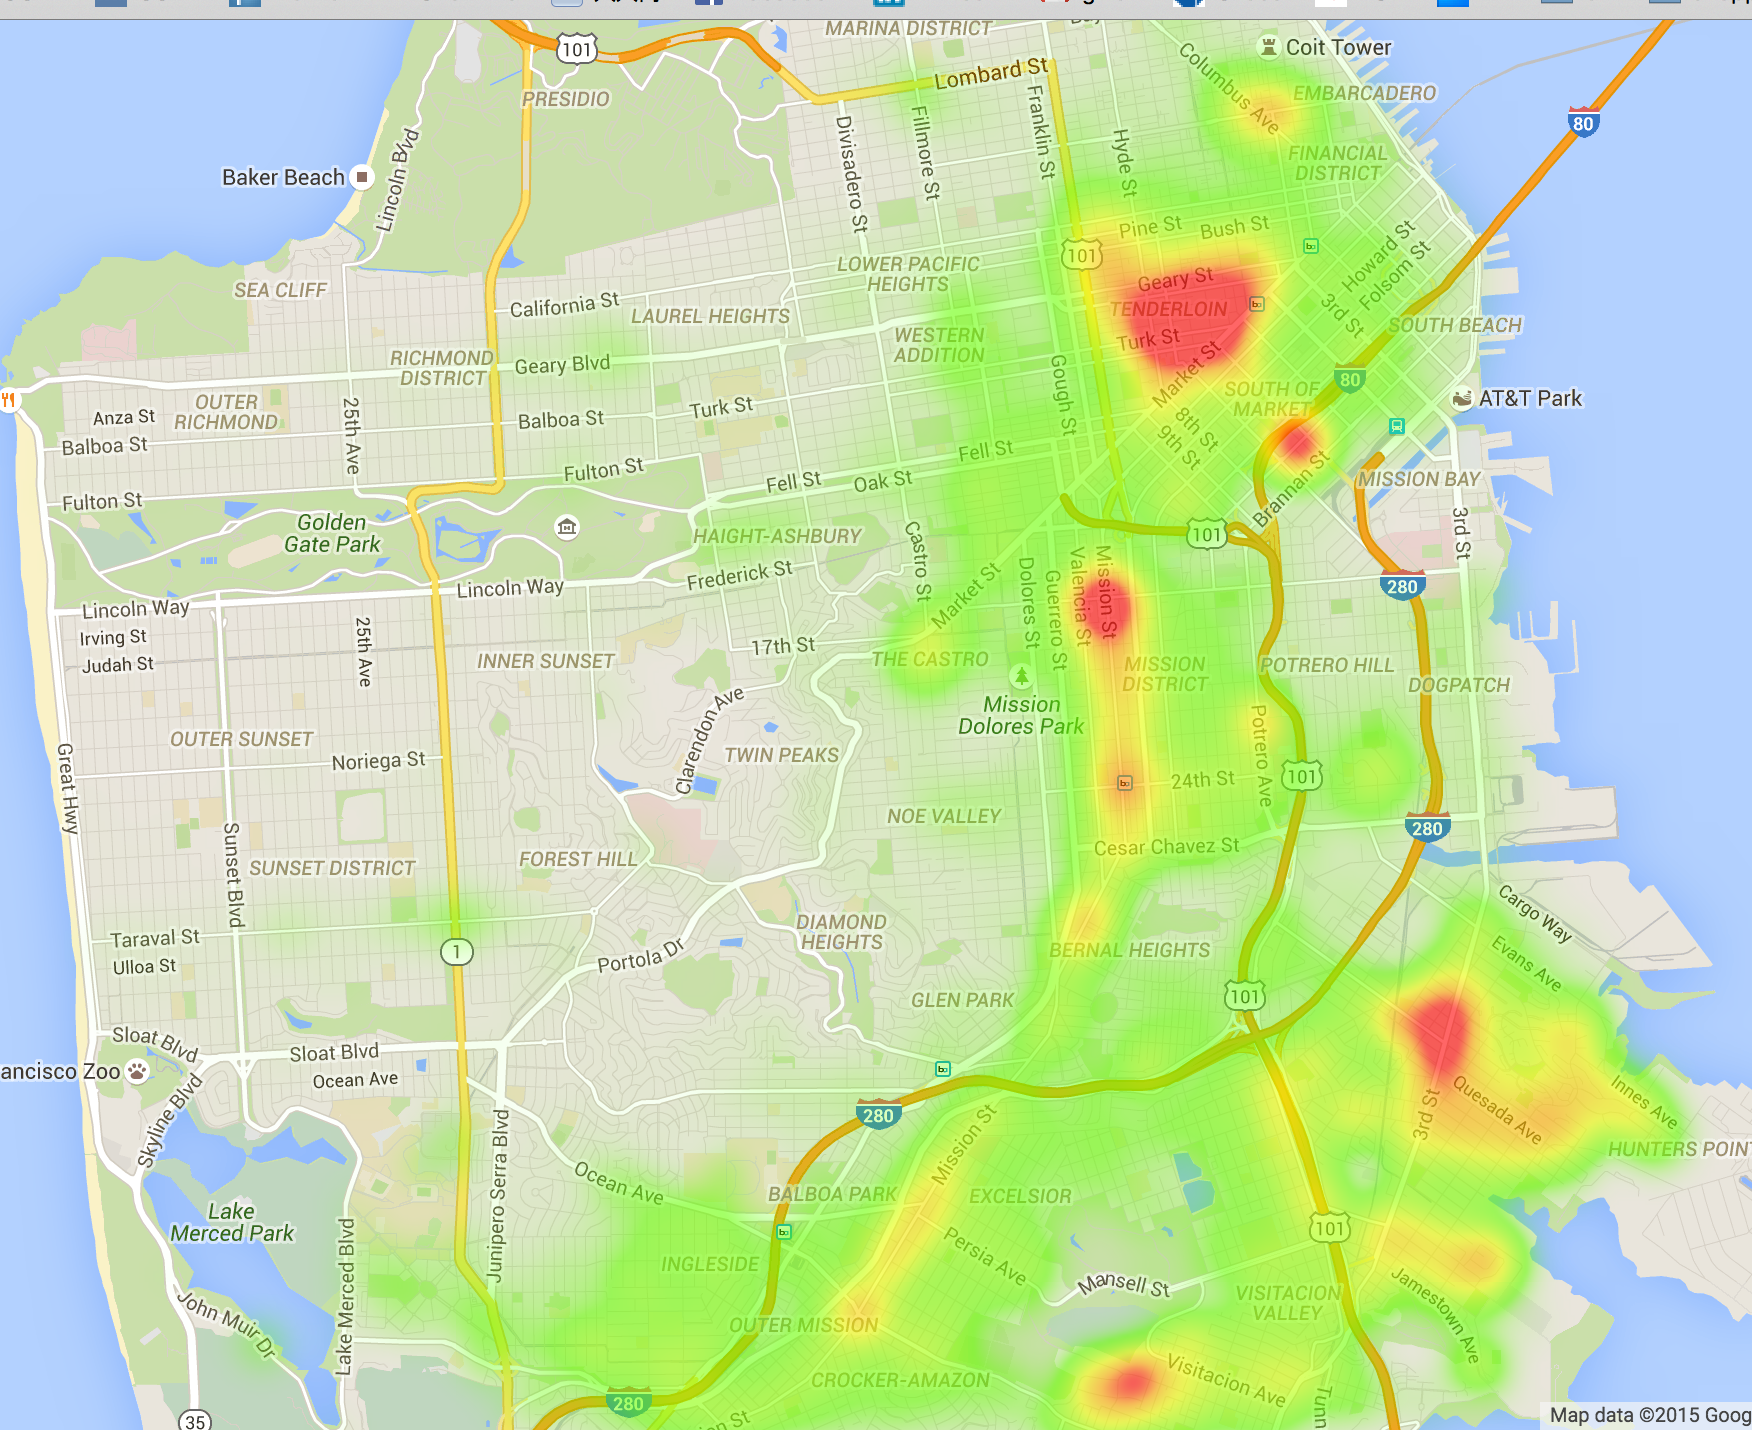
\includegraphics[height=10cm]{ASSAULT_test.png}
\end{center}
\end{p4}

\newpage
\begin{p5}{}
\item{}
For this project we performed a feature selection based on additional location data using decision trees, and used multivariate logistic regression to predict the probability of different crimes to happen for a given time and location. The intuition is that the spatial-temporal distribution of different crimes should follow some pattern, so we should be able to learn some meaningful results from it.\\\\
One observation is that the performance of our classifier was improved largely by adding 10 selected location district and street names into the feature space. Ideally, given enough dataset and with a sufficiently model, features like district and street should be able to learned automatically from latitude and longitude, as they are essentially some patterns of GPS coordinates. But to make the algorithm more practical and the training process fast enough, we took a different approach. We selected the feature ourselves, and chose a simple linear model to learn from. This way we can achieve good results without requiring large amount data and computations.\\\\
One thing to improve is that we can try to design more features from time like "morning", "afternoon", "winter", "summer", and features like landmarks, hotels, rich or poor neighborhood using reverse-geo-encoding services and the GPS coordinates we have. This way our feature selection process will have a larger pool to choose from and may further improve the classification accuracy. Another thing that we can do is to try out more complicated models, though it may require more computation resources.
\end{p5}{}
\begin{p6}{}
\item{}
[1] Kaggle San Francisco Crime Classification https://www.kaggle.com/c/sf-crime
\item{}
[2] Bag of Words model https://en.wikipedia.org/wiki/Bag-of-words model 
\item{}
[3] P. Geurts, D. Ernst., and L. Wehenkel, ``Extremely randomized trees'', Machine Learning, 63(1), 3-42, 2006.

\end{p6}

% --------------------------------------------------------------
%     You don't have to mess with anything below this line.
% --------------------------------------------------------------
 
\end{document}
